%&pdflatex
\documentclass{standalone}
\usepackage{tikz}
\usetikzlibrary{arrows}
\usetikzlibrary{shapes}
\usetikzlibrary{positioning}
\usetikzlibrary{snakes}

\begin{document}

\begin{tikzpicture}
\node[inner sep=0pt] (three1) at (-2,3) {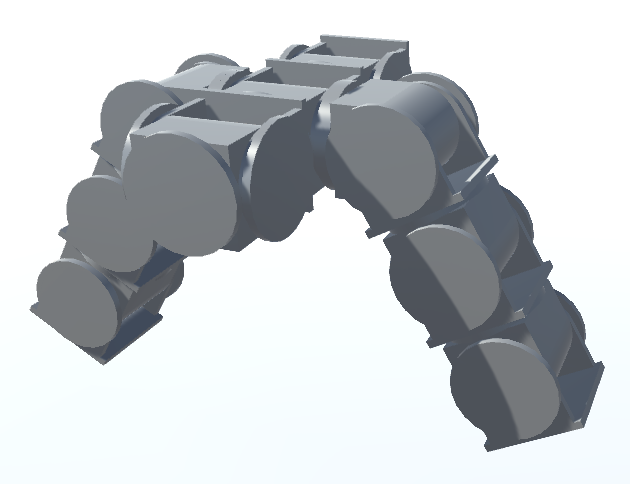
\includegraphics[width=2cm]{../library/unity/cross.png}};
\node[inner sep=0pt] (three2) at (4,3) {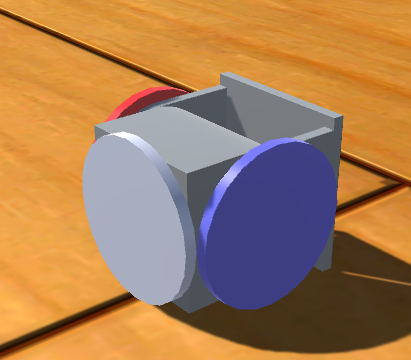
\includegraphics[width=2cm]{../library/unity/singleModule.png}};
\node[inner sep=0pt] (body) at (1,-0.5) {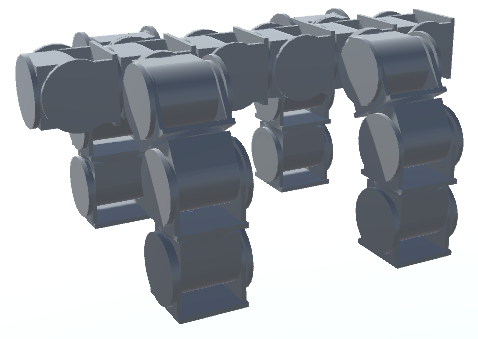
\includegraphics[width=4cm]{../library/unity/lowerBody.png}};
\node[inner sep=0pt] (three3) at (1,3) {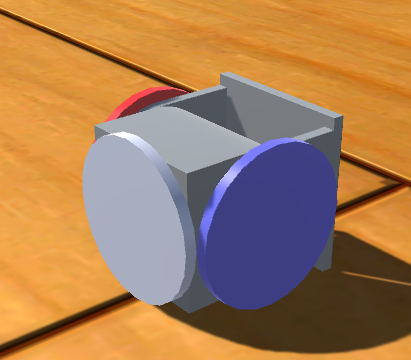
\includegraphics[width=2cm]{../library/unity/singleModule.png}};
%\node[inner sep=0pt] (three4) at (2,-3) {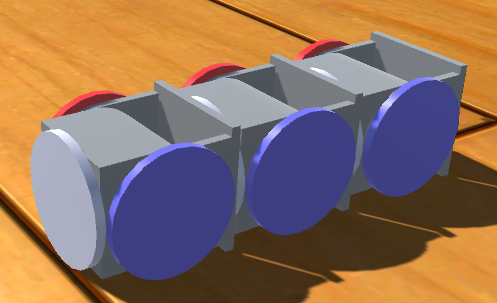
\includegraphics[width=2cm]{../library/unity/threeModules.png}};
\node[inner sep=0pt] (walkbot) at (8,1) {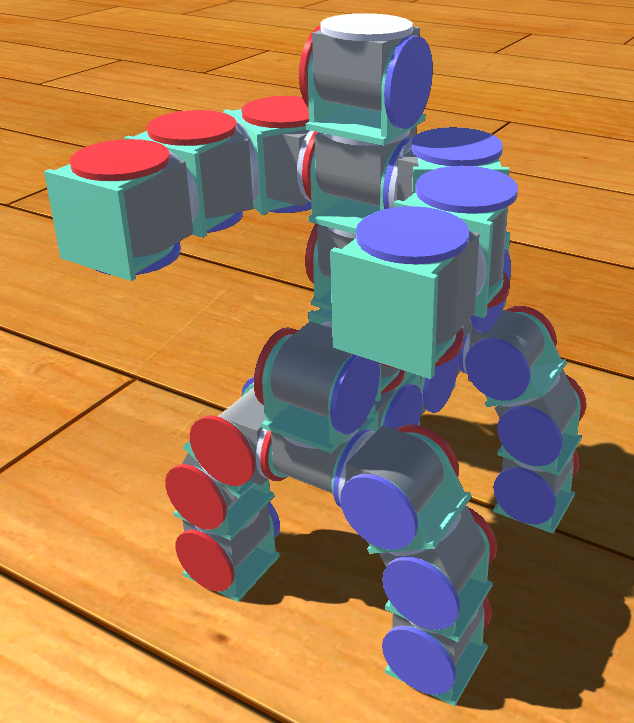
\includegraphics[width=4cm]{../library/unity/centaur.png}};

\draw[->,ultra thick] (three1) -- ([xshift=-1cm]body.north);
\draw[->,ultra thick] (three2) --([xshift=1cm]body.north);
\draw[->,ultra thick] (three3)--(body.north);
%\draw[->,ultra thick] (three4) |-  ([yshift=-0.5cm, xshift=1cm]body.south) -- ([xshift=1cm, yshift=-0.4cm]body.center);
\draw[-implies, double equal sign distance, thick] ([xshift=0.5cm, yshift=1cm]body.east) -- ([xshift=-0.5cm,yshift=-0.5cm]walkbot.west);

\end{tikzpicture}

\end{document}



